\documentclass{thomasClass}
\usepackage[utf8]{inputenc}
\usepackage{multirow}
\usepackage{amssymb}

\title{\textbf{Required Practical 9}
\\Investigation into the effect of a named variable on the rate of respiration of cultures of single-celled organisms
}
\author{Thomas Boxall}
\date{January 2022}

\begin{document}

\maketitle

\section{Method}
\begin{enumerate}
    \item Label five test tubes with numbers 1 to 5
    \item Add $2cm^3$ of yeast solution to each test tube
    \item Place one of each tube into its temperature water bath and allow it to come to temperature (approx. 5 minutes)
    \item Add $2cm^3$ methylene blue to test tube 1, shake the tube for 10 seconds then return to the water bath. Record how long it takes for the solution to turn white
    \item Repeat step 4 for the remaining test tubes.
\end{enumerate}
\section{Null Hypothesis}
The temperature has no effect on the rate of respiration in yeast.

\section{Variables}
\textbf{Independent Variable: }Temperature.\\
\textbf{Dependant Variable: }Rate of reaction.\\
\textbf{Control Variables: }Quantity of yeast and methylene blue; time for yeast to come to temperature; point at which we say the reaction is complete.
\section{Results}
The data obtained from this experiment would be suitable to perform the Spearman's rank correlation coefficient statistic test on, to be able to evaluate the Null Hypothesis.\\
\textit{NB: There are two sets of data, one the class data and one exemplar data as the class yeast solution wasn't behaving as expected.}
\subsection{Class Data}
\subsubsection{Raw data}
\begin{table}[H]
\begin{tabularx}{0.8\textwidth}{c|XXX|XX}
\multicolumn{1}{l}{\multirow{2}{*}{Temperature}} & \multicolumn{3}{c}{Time taken for solution to decolourise (s)} & \multicolumn{1}{l}{} & \multicolumn{1}{l}{} \\
\multicolumn{1}{l}{} & \multicolumn{1}{X}{Exp. 1} & \multicolumn{1}{X}{Exp. 2} & \multicolumn{1}{X}{Exp. 3} & \multicolumn{1}{l}{Mean} & \multicolumn{1}{l}{Rate Of Reaction} \\
\hline
9 & 628 &  &  & 628.00 & 0.001592356688 \\
35 & 660 &  &  & 660.00 & 0.001515151515 \\
43 & 420 & 995 & 1029 & 814.67 & 0.001227495908 \\
51 & 313 & 464 & 612 & 463.00 & 0.002159827214 \\
72 & DNF & DNF &  &  & \multicolumn{1}{c}{}
\end{tabularx}
\end{table}
\subsubsection{Graph}
\begin{figure}[H]
    \centering
    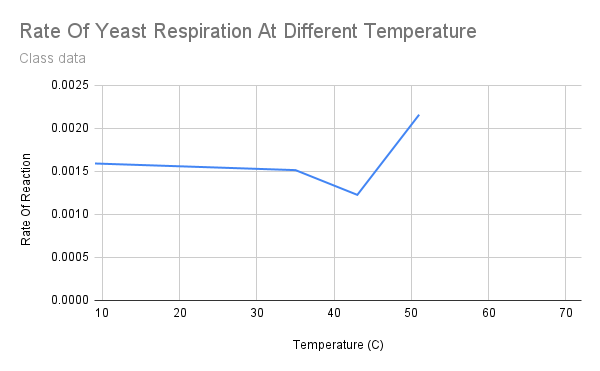
\includegraphics[width=0.5\textwidth]{RPA9-GRAPH1.png}
\end{figure}
\subsubsection{Spearmans Rank Calculations}
\begin{table}[H]
\begin{tabularx}{0.8\textwidth}{XX|XX|XX}
\multicolumn{1}{l}{Temperature} & \multicolumn{1}{l}{Rank} & \multicolumn{1}{l}{Rate of Reaction} & \multicolumn{1}{l}{Rank} & \multicolumn{1}{l}{$D=(R_1-R_2)$} & \multicolumn{1}{l}{$D\times D$} \\
\hline
9 & 1 & 0.001592356688 & 3 & -2 & 4 \\
35 & 2 & 0.001515151515 & 2 & 0 & 0 \\
43 & 3 & 0.001227495908 & 1 & 2 & 4 \\
51 & 4 & 0.002159827214 & 4 & 0 & 0 \\
72 & 5 & \multicolumn{1}{c}{} & 5 & 0 & 0
\end{tabularx}
\end{table}
Sum of $D\times D = 8$\\
$\therefore R_s=0.6$

\subsubsection{Evaluation and Statistical Proof}
From the raw data table, we see that only 1 experiments had a full range of results, one of which is DNF. This lack of results can be put down to dead yeast. However, we can still perform a Spearmans Rank Correlation Coefficient statistical test on the data; the result of which is 0.6. The critical value at P=0.05 with 5 degrees of freedom is 1.00. As the critical value is greater than the result of the statistic test, we can accept the null hypotheses. \\

\subsection{Exemplar Data}
\subsubsection{Raw data}
\begin{table}[H]
\begin{tabularx}{0.8\textwidth}{c|XXX|XX}
\multicolumn{1}{l}{\multirow{2}{*}{Temperature}} & \multicolumn{3}{c}{Time taken for solution to decolourise (s)} & \multicolumn{1}{l}{} & \multicolumn{1}{l}{} \\
\multicolumn{1}{l}{} & \multicolumn{1}{X}{Exp. 1} & \multicolumn{1}{X}{Exp. 2} & \multicolumn{1}{X}{Exp. 3} & \multicolumn{1}{l}{Mean} & \multicolumn{1}{l}{Rate Of Reaction} \\
\hline
20 & 600 & 660 & 600 & 620.00 & 0.001612903226 \\
30 & 348 & 345 & 349 & 347.33 & 0.002879078695 \\
40 & 265 & 260 & 280 & 268.33 & 0.003726708075 \\
50 & 40 & 35 & 42 & 39.00 & 0.02564102564 \\
60 & 105 & 120 & 117 & 114.00 & 0.008771929825
\end{tabularx}
\end{table}
\subsubsection{Graph}
\begin{figure}[H]
    \centering
    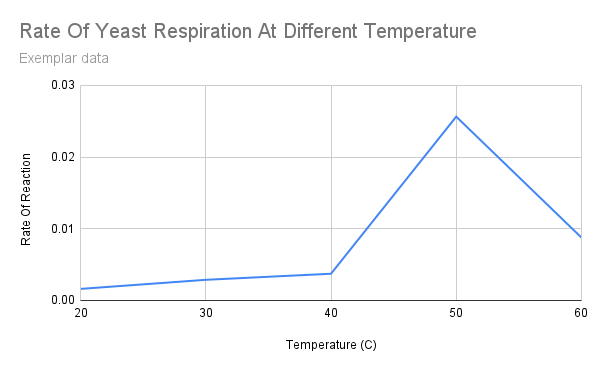
\includegraphics[width=0.5\textwidth]{RPA9-GRAPH2.png}
\end{figure}
\subsubsection{Spearmans Rank Calculations}
\begin{table}[H]
\begin{tabularx}{0.8\textwidth}{XX|XX|XX}
\multicolumn{1}{l}{Temperature} & \multicolumn{1}{l}{Rank} & \multicolumn{1}{l}{Rate of Reaction} & \multicolumn{1}{l}{Rank} & \multicolumn{1}{l}{$D=(R_1-R_2)$} & \multicolumn{1}{l}{$D\times D$} \\
\hline
20 & 1 & 0.001612903226 & 1 & 0 & 0 \\
30 & 2 & 0.002879078695 & 2 & 0 & 0 \\
40 & 3 & 0.003726708075 & 3 & 0 & 0 \\
50 & 4 & 0.02564102564 & 5 & -1 & 1 \\
60 & 5 & 0.008771929825 & 4 & 1 & 1
\end{tabularx}
\end{table}
Sum of $D\times D = 2$\\
$\therefore R_s=0.9$
\subsubsection{Evaluation and Statistical Proof}
This experiment had a full set of results and as a result we can assume it has a higher level of accuracy. The result of the Spearmans Rank Correlation Coefficient statistical test is 0.9. As this is less than the critical value at 5 degrees of freedom, we can accept the null hypothesis.
\end{document}
